\documentclass[11pt,a4paper]{article}
\usepackage[margin=23mm]{geometry}
% Lighter Overleaf build: choose pdfLaTeX, not XeLaTeX.
\usepackage[T1,T2A]{fontenc}
\usepackage[utf8]{inputenc}
\usepackage[english,russian]{babel}
\usepackage{amsmath,amssymb}
\usepackage{graphicx,booktabs,microtype}
\usepackage[unicode,hidelinks]{hyperref}
\setlength{\emergencystretch}{3em}

\title{Классификация фокальной дистонии по данным МРТ}
\author{Рада Лихачева}
\date{}
\begin{document}
\maketitle
\begin{abstract}

В работе рассматривается задача классификации фокальной дистонии по структурным магнитно-резонансным изображениям головного мозга с использованием предобученной модели BrainIAC. Цель исследования: адаптировать модель для различения пациентов с дистонией верхней конечности и здоровых участников на открытом наборе данных OpenNeuro ds006395. Исследование предусматривает дообучение энкодера и сравнение с классификатором на признаках замороженной модели. В выполненном базовом эксперименте на 66 участниках использованы 768-мерные представления BrainIAC и логистическая регрессия; при стратифицированной пятикратной кросс-валидации получены сбалансированная точность 0,562 и ROC-AUC 0,569. Эти значения рассматриваются как предварительная точка отсчета; устойчивое преимущество над случайным уровнем пока не установлено. Дальнейшие эксперименты направлены на оценку вклада дообучения в качество и устойчивость классификации при ограниченном объеме данных.

\textbf{Ключевые слова:} фокальная дистония; структурная МРТ; BrainIAC; перенос обучения; классификация.

\end{abstract}
\section{Введение}

Дистония - двигательное расстройство, характеризующееся устойчивыми или периодически возникающими патологическими движениями, позами либо их сочетанием \cite{ref29}. При фокальной форме нарушения ограничены одной областью тела; в настоящей работе рассматривается дистония верхней конечности. Поиск количественных нейровизуализационных признаков заболевания мотивирует разработку методов автоматической классификации пациентов и здоровых участников. Структурная магнитно-резонансная томография позволяет исследовать анатомические характеристики головного мозга, однако выделение признаков, пригодных для индивидуального предсказания, остается сложной задачей. Цель настоящего исследования - адаптация предобученной модели BrainIAC для классификации дистонии верхней конечности по T1-взвешенным изображениям.

Существующие исследования используют морфометрические характеристики коры и подкорковых структур, показатели диффузии и функциональной связности. При этом результаты зависят от клинической формы и выбранного способа анализа. Так, de Faria и соавторы \cite{ref01} не обнаружили значимых структурных различий между пациентами с дистонией верхней конечности и здоровыми участниками, тогда как анализ стриарных компартментов выявил особенности, различающиеся между подтипами фокальной дистонии \cite{ref03}. Отдельное направление связано с непосредственной классификацией изображений: модель DystoniaNet использует трехмерную сверточную сеть для распознавания дистонии по структурной МРТ \cite{ref06}. Таким образом, существующая литература обосновывает применение машинного обучения, но не устанавливает универсальную переносимость полученных решений между формами заболевания.

Основные ограничения этой задачи связаны с небольшими размеченными выборками, высокой размерностью изображений и неоднородностью клинических групп. Наличие групповых различий само по себе не гарантирует точной классификации нового участника, а их отсутствие не исключает информативности многомерного представления. Кроме того, при малом числе наблюдений качество существенно зависит от разбиения данных, а утечки при обработке или выборе признаков могут приводить к завышенным оценкам \cite{ref20,ref22}. Поэтому результаты, полученные для других форм дистонии и при иных процедурах тестирования, требуют отдельной проверки на целевой выборке.

В настоящей работе рассматривается перенос обучения с использованием BrainIAC - модели анализа МРТ головного мозга, основанной на трехмерном Vision Transformer и контрастивном самообучении \cite{ref09}. Предлагается адаптировать ее представления к различению пациентов с дистонией верхней конечности и здоровых участников и сопоставить дообучение с линейным классификатором на признаках замороженного энкодера. Выбор такого подхода позволяет использовать знания, полученные при предварительном обучении на крупной коллекции МРТ, и проверить необходимость обновления представлений на целевых данных. При этом преимущество дообучения не предполагается заранее: изменение предобученных признаков может снижать обобщающую способность модели \cite{ref19}.

Исследование сосредоточено на сравнении режимов адаптации BrainIAC в едином протоколе классификации. Для вычислительных экспериментов выбран открытый набор OpenNeuro ds006395; используются структурные T1-взвешенные изображения пациентов с дистонией верхней конечности и здорового контроля. Предусматриваются проверка качества изображений, согласованная предобработка, обучение классификаторов и оценка на одинаковых разбиениях по участникам. Подбор гиперпараметров выполняется внутри обучающих подвыборок, а основными метриками служат сбалансированная точность и площадь под ROC-кривой. Такое сравнение направлено на оценку вклада дообучения и устойчивости классификации при ограниченном объеме данных.

\section{Обзор литературы}

\subsection{Структурные и функциональные признаки дистонии}

Нейровизуализационные исследования дистонии рассматривают изменения корковых, подкорковых структур и связей между ними. Однако обнаруживаемые особенности зависят от клинической формы, модальности МРТ и способа обработки. В исследовании структурных изменений при цервикальной и генерализованной дистонии анализировались толщина коры, объемы и форма подкорковых структур \cite{ref05}. Его результаты характеризуют эти клинические группы, но не устанавливают универсальный признак, одинаково применимый ко всем формам дистонии.

Для настоящей работы особенно значимо исследование de Faria и соавт. по дистонии верхней конечности \cite{ref01}. Авторы проанализировали структурные T1-взвешенные изображения и диффузионные данные 28 пациентов и 29 здоровых участников. После морфометрического и диффузионного анализа значимых межгрупповых различий обнаружено не было. Этот результат ограничивает ожидания относительно выраженности структурного сигнала, но сам по себе не исключает классификацию на основе сочетания нескольких признаков. Проверка гипотезы о средних групповых различиях и оценка предсказания для нового участника являются различными статистическими задачами.

В анализе 91 участника, включавшем дистонию верхней конечности, цервикальную дистонию и контроль, выявлены зависимые от подтипа особенности стриарных компартментов и белого вещества \cite{ref03}. Отдельная работа исследует объемы таламуса и его подразделений на данных ds006395 \cite{ref04}. Эти результаты показывают важность локальных представлений и клинической неоднородности. При этом повторные анализы одного открытого набора нельзя считать независимыми внешними подтверждениями. Кроме того, признаки диффузионной МРТ не доступны автоматически модели, использующей только T1-изображения.

Функциональные исследования расширяют представление о сетевых изменениях. Guo и соавт. сопоставили морфометрию и функциональную связность у 35 пациентов с цервикальной дистонией и 28 здоровых участников \cite{ref02}. Другие авторы использовали функциональную связность и региональную однородность для SVM-классификации \cite{ref07,ref08}. Эти исследования обосновывают интерес к индивидуальным предсказаниям, но их результаты не являются прямым ориентиром качества классификации ULD по структурной T1-МРТ: отличаются заболевание, модальность и протокол оценки.

\subsection{Прямая классификация по МРТ}

Ключевой работой по классификации дистонии на структурных изображениях является DystoniaNet \cite{ref06}. В ней трехмерная сверточная сеть обучалась извлекать признаки непосредственно из МРТ и формировать решение о принадлежности к клинической группе. Работа показывает, что постановка классификации дистонии по структурным изображениям уже существует; применение нейросети к этой задаче само по себе не составляет новизну.

Перенос опубликованного качества DystoniaNet на настоящую задачу ограничен различиями клинических форм, выборок и схем тестирования. В частности, сообщаемое авторами высокое качество на дополнительной пациентской выборке с возможностью направления на дополнительное обследование нельзя трактовать как обычную бинарную accuracy на смешанной выборке пациентов и контроля. Сравнение с новой моделью должно проводиться при одинаковых классах, метриках и независимых тестовых объектах.

Таким образом, DystoniaNet является ближайшим предметным предшественником. Прямое экспериментальное сравнение требует общей выборки, одинаковых целевых классов и процедуры оценки.

\subsection{Предобученные модели и адаптация к новой задаче}

Ограниченное количество размеченных МРТ мотивирует перенос представлений, обученных на более крупных коллекциях. Ранние подходы включают Med3D/MedicalNet, использующий предобучение трехмерных сетей на нескольких медицинских задачах \cite{ref15}, и Models Genesis, где сеть обучается восстанавливать преобразованные фрагменты изображений \cite{ref16}. Эти работы различаются целью обучения и исходными данными; их результаты обосновывают подход к переносу, но не доказывают эффективность для дистонии.

Трансформерные архитектуры развивают этот подход через представление изображения в виде последовательности пространственных патчей \cite{ref18}. В медицинской визуализации Swin UNETR использует специальные задачи самообучения для трехмерных изображений \cite{ref17}, а BrainSegFounder сочетает этапы предобучения для нейровизуализационной сегментации \cite{ref10}. Успех сегментации не равнозначен успешной классификации клинических групп, поэтому эти модели рассматриваются как методический контекст и возможные будущие альтернативы.

Основой настоящего проекта выбрана BrainIAC \cite{ref09}. В журнальной версии 2026 года модель использует трехмерный ViT-B и контрастивное самообучение; авторы сравнивают адаптацию к нескольким задачам, включая linear probing и сквозное дообучение. Здесь важно опираться именно на журнальную версию: ранний препринт описывал иную конфигурацию модели и меньший набор задач. Оценка BrainIAC на исходных задачах не устанавливает ее качество на ULD.

Современные альтернативы включают AnatCL, учитывающую анатомическую информацию при контрастивном обучении \cite{ref11}, 3DINO с самодистилляцией на разнородных объемных данных \cite{ref12} и BrainDINO, использующую срезовые представления и замороженный энкодер \cite{ref13}. OpenMind предлагает открытые данные и стандартизированные условия изучения трехмерного самообучения \cite{ref14}. Эти работы показывают разнообразие переносимых представлений и необходимость сопоставимых условий оценки. В настоящем исследовании основное сравнение ограничено режимами адаптации BrainIAC.

Дообучение не гарантирует улучшения относительно замороженного энкодера. Kumar и соавт. показывают, что обновление предобученных представлений при сдвиге распределения может ухудшать обобщение \cite{ref19}. Поэтому в нашей работе frozen baseline сохраняется как обязательная точка сравнения. Сравнение обучения головы, частичного и полного дообучения формирует проверяемую экспериментальную ось; преимущество одного режима должно быть установлено на целевой выборке.

\subsection{Малые выборки, утечки данных и оценка качества}

При небольшом числе участников оценка качества чувствительна к выбору разбиения. Varoquaux анализирует неопределенность кросс-валидации на малых выборках \cite{ref20}, а Vabalas и соавт. исследуют влияние процедуры валидации на оценку алгоритмов \cite{ref24}. Поэтому единственное удачное разбиение не является достаточным подтверждением преимущества. При сравнении режимов адаптации нужно использовать одни и те же внешние folds и отделять подбор гиперпараметров от итоговой оценки.

Wen и соавт. проводят воспроизводимую оценку классификации по T1-МРТ и демонстрируют проблему утечек \cite{ref21}. Отдельное экспериментальное исследование показывает искажение результатов при распределении срезов одного человека между обучением и тестированием \cite{ref27}. Аналогичные проблемы отбора признаков и обработки данных исследуются в работах по коннектомному прогнозированию \cite{ref22}. В нашем протоколе все изображения и производные одного участника должны оставаться внутри одного fold, а обучаемые преобразования должны оцениваться только по обучающей части.

Возраст, пол, размеры мозга и технические характеристики изображений могут быть источниками предсказательного сигнала, не совпадающего с клиническими различиями. Работа Snoek и соавт. обосновывает необходимость контроля конфаундеров внутри процедуры валидации \cite{ref23}. Исследование воспроизводимости эмбеддингов при сканировании одних участников на разных сканерах представляет дополнительный современный контекст технической вариабельности \cite{ref28}.

Для сопоставления качества со случайным уровнем могут применяться перестановочные тесты \cite{ref25}. При перестановке меток необходимо повторять весь обучаемый протокол, включая подбор гиперпараметров, если он проводился в основном эксперименте. Работа Marek и соавт. подчеркивает проблему воспроизводимости слабых межиндивидуальных brain–phenotype ассоциаций \cite{ref26}, однако ее вывод о тысячах участников нельзя трактовать как универсальный минимальный объем для любой задачи классификации дистонии.

\subsection{Вывод и место настоящей работы}

В литературе уже представлены классификация дистонии по МРТ, анализ структурных особенностей ULD и перенос предобученных нейровизуализационных моделей. Следовательно, предполагаемый вклад настоящей работы следует формулировать на уровне конкретной адаптации и экспериментальной проверки: классификация ULD и здорового контроля по T1-МРТ с использованием BrainIAC и сравнением режимов обучения в едином протоколе.

Рабочая гипотеза состоит в том, что адаптация предобученных представлений к целевой клинической выборке может изменить качество классификации по сравнению с обучением линейного классификатора на замороженных признаках. Направление изменения заранее не фиксируется как установленный факт. Вклад исследования связывается со сравнением режимов адаптации на целевой задаче в едином протоколе оценки.

\section{Постановка задачи}

Рассматривается задача бинарной классификации пациентов с дистонией верхней конечности и здоровых участников по структурным T1-взвешенным МРТ головного мозга. Требуется построить классификатор на основе предобученной модели BrainIAC и сравнить использование замороженных представлений с адаптацией энкодера к целевой задаче.

\subsection{Данные и обозначения}

Пусть задана выборка
\[
\mathcal{D}=\{(x_i,y_i)\}_{i=1}^{n},
\]
где \(x_i\) - трехмерное T1-взвешенное изображение одного участника, а \(y_i\in\{0,1\}\) - метка класса: \(y_i=0\) для здорового контроля и \(y_i=1\) для пациента с дистонией верхней конечности. В предварительном эксперименте использованы \(n=66\) участников: 37 здоровых и 29 пациентов. Участники с цервикальной дистонией в эту постановку не включаются.

Обозначим через \(T\) процедуру предобработки изображения, а через \(g_\theta\) - энкодер BrainIAC с параметрами \(\theta\). Через \(S_{\mathrm{tr}}\) обозначается стандартизация признаков, параметры которой оцениваются на обучающей части. Изображению сопоставляется вектор признаков
\[
z_i=S_{\mathrm{tr}}\!\left(g_\theta(T(x_i))\right)\in\mathbb{R}^{768}.
\]

Линейный классификатор определяет вероятность положительного класса:
\[
p_i=p_{\theta,w,b}(y_i=1\mid x_i)
=\sigma(w^\top z_i+b),
\qquad
\sigma(t)=\frac{1}{1+\exp(-t)},
\]
где \(w\in\mathbb{R}^{768}\) и \(b\in\mathbb{R}\) - обучаемые параметры. В базовом эксперименте стандартизация применяется к признакам замороженного энкодера. Для сквозного дообучения может использоваться тождественное преобразование \(S_{\mathrm{tr}}=I\).

\subsection{Критерий обучения}

В качестве внутреннего критерия рассматривается взвешенная бинарная кросс-энтропия с L2-регуляризацией коэффициентов классификатора:
\[
Q(\theta,w,b;\mathcal{D}_{\mathrm{tr}})
=
-\frac{1}{\sum_{i\in I_{\mathrm{tr}}}a_{y_i}}
\sum_{i\in I_{\mathrm{tr}}}
a_{y_i}
\left[
y_i\log p_i+(1-y_i)\log(1-p_i)
\right]
+\frac{\lambda}{2}\|w\|_2^2.
\]

Здесь \(I_{\mathrm{tr}}\) - индексы обучающих участников, \(a_0,a_1>0\) - веса классов, вычисляемые по обучающей выборке, а \(\lambda>0\) определяет силу регуляризации. Нормировка записана для математического описания метода; соответствие \(\lambda\) параметру \(C\) зависит от нормировки функции потерь в реализации.

В базовом эксперименте параметры энкодера фиксируются на предобученных значениях \(\theta_0\), и решается задача
\[
(w^*,b^*)=
\operatorname*{arg\,min}_{w,b}
Q(\theta_0,w,b;\mathcal{D}_{\mathrm{tr}}).
\]

На следующем этапе предполагается оптимизация также выбранного подмножества параметров энкодера:
\[
(\theta^*,w^*,b^*)=
\operatorname*{arg\,min}_{\theta\in\Theta_{\mathrm{adapt}},\,w,b}
Q(\theta,w,b;\mathcal{D}_{\mathrm{tr}}),
\]
где \(\Theta_{\mathrm{adapt}}\) задает режим адаптации: обновление выбранных блоков или всего энкодера с инициализацией \(\theta_0\). Дообучение энкодера является планируемой частью исследования.

\subsection{Валидация и внешние критерии}

Основные внешние критерии - сбалансированная точность и площадь под ROC-кривой. Для положительного класса «дистония» сбалансированная точность определяется как
\[
\mathrm{BA}=
\frac{1}{2}
\left(
\frac{TP}{TP+FN}
+
\frac{TN}{TN+FP}
\right).
\]

Дополнительно оцениваются accuracy, чувствительность, специфичность и матрица ошибок. Для бинарного решения в базовой логистической регрессии применяется стандартный порог 0,5; ROC-AUC оценивает ранжирование по вероятностям.

Предварительная оценка выполнена с помощью стратифицированной пятикратной кросс-валидации по участникам. Все изображения, производные данные и аугментации одного человека должны оставаться внутри одного разбиения. Для последующего сравнения режимов используются одинаковые внешние разбиения; подбор гиперпараметров и ранняя остановка выполняются только внутри обучающей части.

Ограничения исследования включают небольшой объем выборки, использование одной модальности и отсутствие независимой внешней тестовой когорты. Качество внутри данной выборки не интерпретируется как подтверждение клинической диагностической готовности.

\section{Базовый вычислительный эксперимент}

\subsection{Цель и конфигурация}

Цель базового эксперимента - получить исходное качество классификации ULD и здорового контроля при использовании предобученных признаков BrainIAC без изменения весов энкодера. Этот результат служит точкой отсчета для дальнейшего дообучения.

Использованы T1-взвешенные изображения 66 участников OpenNeuro ds006395 \cite{dataset}: 29 пациентов с дистонией верхней конечности и 37 здоровых участников. Предварительная обработка включала приведение к ориентации RAS, изменение размера до \(96\times96\times96\) вокселей и Z-нормализацию интенсивностей по ненулевым вокселям. Удаление тканей вне мозга, регистрация в стандартное пространство и N4-коррекция в этом запуске не выполнялись.

Для каждого изображения замороженный BrainIAC формировал 768-мерное представление. Классификация проводилась с использованием стандартизации признаков и логистической регрессии. Применялись \(C=0{,}1\), балансировка весов классов и ограничение в 3000 итераций оптимизации. Использовался StratifiedKFold с пятью разбиениями, перемешиванием и random\_state=42.

Вектор признаков извлекался как первый токен патча на выходе энкодера, а не CLS-токен. StandardScaler обучался внутри каждого фолда. ROC-AUC рассчитан по объединенным out-of-fold вероятностям, а не усреднением значений отдельных фолдов.

\subsection{Предварительные результаты}

% Generated from results/metrics.json; historical notebook results.
\begin{center}
\begin{tabular}{lr}
\toprule
Метрика & Значение \\
\midrule
Accuracy & 0,576 \\
Balanced accuracy & 0,562 \\
ROC-AUC & 0,569 \\
\bottomrule
\end{tabular}
\end{center}


Матрица ошибок, сохраненная в выводе запуска:

% Generated from results/metrics.json; row/column order HC, ULD.
\begin{center}
\begin{tabular}{lrr}
\toprule
Истинный класс & Предсказан HC & Предсказан ULD \\
\midrule
HC & 25 & 12 \\
ULD & 16 & 13 \\
\bottomrule
\end{tabular}
\end{center}


\begin{figure}[htbp]
\centering
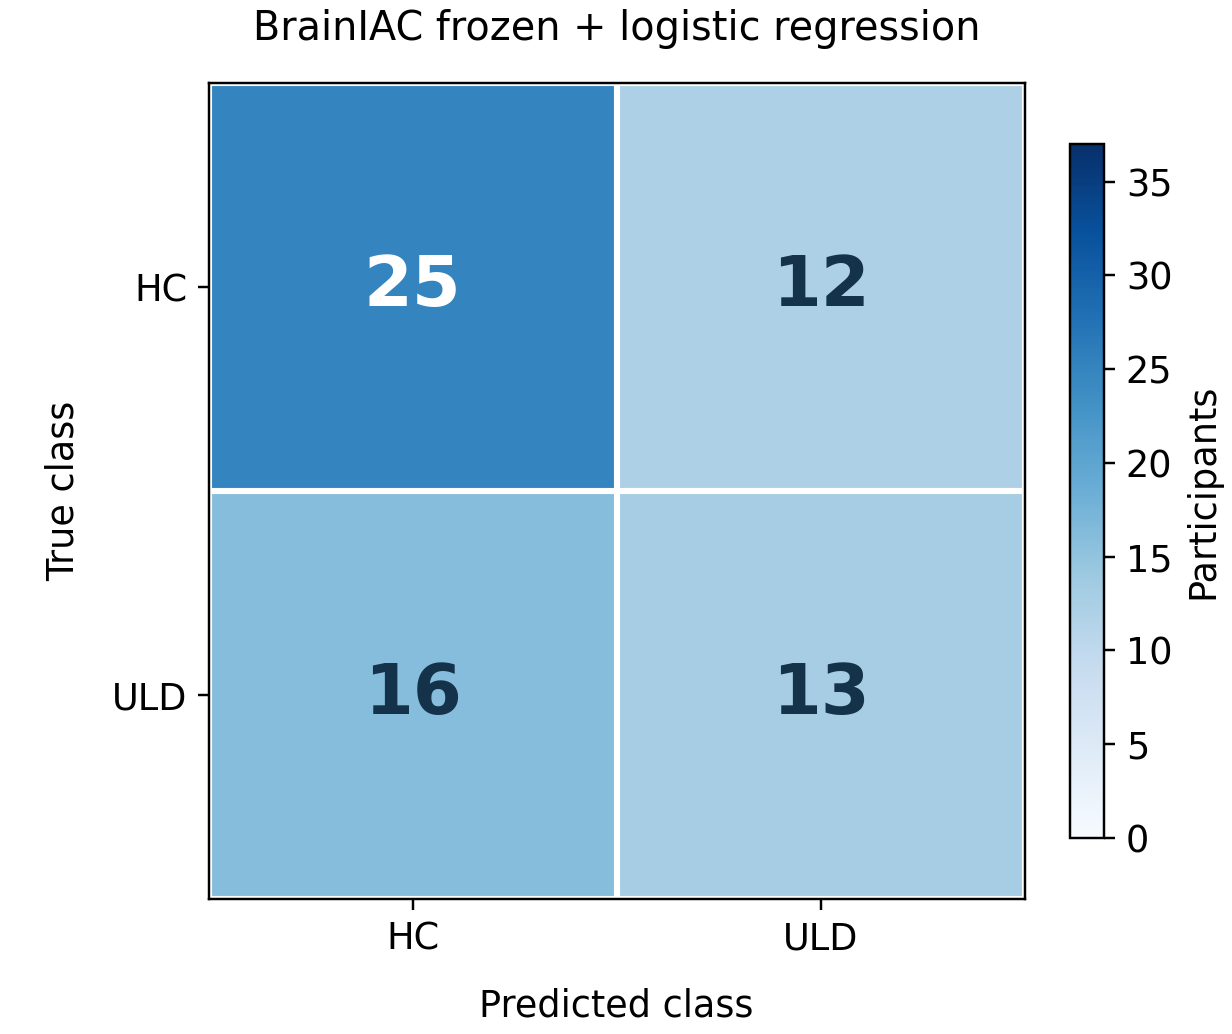
\includegraphics[width=0.60\linewidth]{article/figures/confusion_matrix.png}
\caption{Матрица ошибок базового классификатора. Строки - истинные классы, столбцы - предсказания.}
\end{figure}

При положительном классе ULD чувствительность составляет \(13/29\approx0{,}448\), а специфичность - \(25/37\approx0{,}676\). Для сравнения, постоянное предсказание HC на этой выборке дает accuracy \(37/66\approx0{,}561\) и balanced accuracy \(0{,}5\). Это аналитическая контрольная величина, а не результат отдельно запущенного DummyClassifier.

Полученные значения близки к случайному уровню. Статистическая значимость отличия от нулевого уровня и устойчивость результатов по повторным разбиениям пока не установлены. Поэтому эксперимент рассматривается как предварительный baseline, подтверждающий работоспособность цепочки извлечения признаков и обучения классификатора, но не как свидетельство надежной диагностической классификации.

\section{Обсуждение и дальнейшая работа}

Предварительный эксперимент демонстрирует работоспособность цепочки извлечения признаков и обучения классификатора, однако не подтверждает надежного разделения клинических групп. Чувствительность к пациентам ниже специфичности к контролю, а accuracy лишь немного превышает результат постоянного предсказания наиболее частого класса. В этой ситуации основные выводы следует строить по сбалансированной точности, ROC-AUC и оценке неопределенности.

Ограничения включают малый размер выборки, упрощенную предобработку и отсутствие внешней тестовой когорты. Кроме того, еще не выполнены анализ чувствительности к разбиениям и перестановочная проверка. Отдельной проверки требуют совместимость загруженных весов с архитектурой и способ извлечения признаков.

Дальнейшая работа предусматривает согласование предобработки с требованиями модели и сравнение замороженного энкодера с дообучением выбранных блоков. При изменении предобработки baseline необходимо пересчитать в тех же условиях: это позволит отделить эффект обработки изображений от эффекта адаптации. Сравнение планируется проводить на одинаковых внешних разбиениях по участникам, с подбором параметров и ранней остановкой только внутри обучающей части.

Окончательный вывод о сравнении режимов адаптации будет сформулирован после выполнения запланированных экспериментов.
% Generated from article/references.bib; no Biber required.
\begin{thebibliography}{99}
\small
\bibitem{ref01}
\begin{otherlanguage}{english}
{de Faria}, Danilo Donizete et al. \textit{{Structural brain analysis in focal upper limb dystonia}}. Scientific Reports. 2026. DOI: \url{10.1038/s41598-026-39542-z}.
\end{otherlanguage}
\bibitem{ref02}
\begin{otherlanguage}{english}
Guo, Qingwei; Luo, Yaru; Du, Naixuan et al. \textit{{Multimodal MRI reveals structural and functional alterations in isolated cervical dystonia: associations with motor severity and affective symptoms}}. Frontiers in Neurology. 2026. DOI: \url{10.3389/fneur.2026.1771144}.
\end{otherlanguage}
\bibitem{ref03}
\begin{otherlanguage}{english}
{Marques Paulo}, Artur Jos{\'e}; Waugh, Jeff L.; Winkler, Anderson M. et al. \textit{{Striatal compartment and white matter alterations in focal dystonia Subtypes: An MRI study}}. Parkinsonism \& Related Disorders. 2025. DOI: \url{10.1016/j.parkreldis.2025.108096}.
\end{otherlanguage}
\bibitem{ref04}
\begin{otherlanguage}{english}
Yi\u{g}it, H\"{u}seyin; G\"{o}ko\u{g}lu, Abdulkerim. \textit{{Distinct thalamic volumetric profiles in cervical and upper limb dystonia}}. Arquivos de Neuro-Psiquiatria. 2026. DOI: \url{10.1055/s-0046-1825521}.
\end{otherlanguage}
\bibitem{ref05}
\begin{otherlanguage}{english}
Wu, Yunhao; Wang, Tao; Ding, Qiong et al. \textit{{Cortical and Subcortical Structural Abnormalities in Patients With Idiopathic Cervical and Generalized Dystonia}}. Frontiers in Neuroimaging. 2022. DOI: \url{10.3389/fnimg.2022.807850}.
\end{otherlanguage}
\bibitem{ref06}
\begin{otherlanguage}{english}
Valeriani, Davide; Simonyan, Kristina. \textit{{A microstructural neural network biomarker for dystonia diagnosis identified by a DystoniaNet deep learning platform}}. Proceedings of the National Academy of Sciences. 2020. DOI: \url{10.1073/pnas.2009165117}.
\end{otherlanguage}
\bibitem{ref07}
\begin{otherlanguage}{english}
Li, Zhihao; Prudente, Cec\'{i}lia N.; Stilla, Randall et al. \textit{{Alterations of resting-state fMRI measurements in individuals with cervical dystonia}}. Human Brain Mapping. 2017. DOI: \url{10.1002/hbm.23651}.
\end{otherlanguage}
\bibitem{ref08}
\begin{otherlanguage}{english}
Pan, Pan; Wei, Shubao; Ou, Yangpan et al. \textit{{Reduced Global-Brain Functional Connectivity and Its Relationship With Symptomatic Severity in Cervical Dystonia}}. Frontiers in Neurology. 2020. DOI: \url{10.3389/fneur.2019.01358}.
\end{otherlanguage}
\bibitem{ref09}
\begin{otherlanguage}{english}
Tak, Divyanshu; Garomsa, Biniam A.; Zapaishchykova, Anna et al. \textit{{A generalizable foundation model for analysis of human brain MRI}}. Nature Neuroscience. 2026. DOI: \url{10.1038/s41593-026-02202-6}.
\end{otherlanguage}
\bibitem{ref10}
\begin{otherlanguage}{english}
Cox, Joseph; Liu, Peng; Stolte, Skylar E. et al. \textit{{BrainSegFounder: Towards 3D foundation models for neuroimage segmentation}}. Medical Image Analysis. 2024. DOI: \url{10.1016/j.media.2024.103301}.
\end{otherlanguage}
\bibitem{ref11}
\begin{otherlanguage}{english}
Barbano, Carlo Alberto; Brunello, Matteo; Dufumier, Benoit et al. \textit{{Anatomical foundation models for brain MRIs}}. Pattern Recognition Letters. 2026. DOI: \url{10.1016/j.patrec.2025.11.028}.
\end{otherlanguage}
\bibitem{ref12}
\begin{otherlanguage}{english}
Xu, Tony; Hosseini, Sepehr; Anderson, Chris et al. \textit{{A generalizable 3D framework and model for self-supervised learning in medical imaging}}. npj Digital Medicine. 2025. DOI: \url{10.1038/s41746-025-02035-w}.
\end{otherlanguage}
\bibitem{ref13}
\begin{otherlanguage}{english}
Wu, Yizhou; Wang, Shansong; Li, Yuheng et al. \textit{{BrainDINO: A Brain MRI Foundation Model for Generalizable Clinical Representation Learning}}. 2026. \url{https://arxiv.org/abs/2604.27277}.
\end{otherlanguage}
\bibitem{ref14}
\begin{otherlanguage}{english}
Wald, Tassilo; Ulrich, Constantin; Suprijadi, Jonathan et al. \textit{{An OpenMind for 3D Medical Vision Self-supervised Learning}}. Proceedings of the IEEE/CVF International Conference on Computer Vision. 2025. \url{https://openaccess.thecvf.com/content/ICCV2025/html/Wald_An_OpenMind_for_3D_Medical_Vision_Self-supervised_Learning_ICCV_2025_paper.html}.
\end{otherlanguage}
\bibitem{ref15}
\begin{otherlanguage}{english}
Chen, Sihong; Ma, Kai; Zheng, Yefeng. \textit{{Med3D: Transfer Learning for 3D Medical Image Analysis}}. 2019. \url{https://arxiv.org/abs/1904.00625}.
\end{otherlanguage}
\bibitem{ref16}
\begin{otherlanguage}{english}
Zhou, Zongwei; Sodha, Vatsal; Pang, Jiaxuan et al. \textit{{Models Genesis}}. Medical Image Analysis. 2021. DOI: \url{10.1016/j.media.2020.101840}.
\end{otherlanguage}
\bibitem{ref17}
\begin{otherlanguage}{english}
Tang, Yucheng; Yang, Dong; Li, Wenqi et al. \textit{{Self-Supervised Pre-Training of Swin Transformers for 3D Medical Image Analysis}}. Proceedings of the IEEE/CVF Conference on Computer Vision and Pattern Recognition. 2022. DOI: \url{10.1109/CVPR52688.2022.02007}.
\end{otherlanguage}
\bibitem{ref18}
\begin{otherlanguage}{english}
Dosovitskiy, Alexey et al. \textit{{An Image is Worth 16x16 Words: Transformers for Image Recognition at Scale}}. International Conference on Learning Representations. 2021. \url{https://arxiv.org/abs/2010.11929}.
\end{otherlanguage}
\bibitem{ref19}
\begin{otherlanguage}{english}
Kumar, Ananya; Raghunathan, Aditi; Jones, Robbie et al. \textit{{Fine-Tuning can Distort Pretrained Features and Underperform Out-of-Distribution}}. International Conference on Learning Representations. 2022. \url{https://arxiv.org/abs/2202.10054}.
\end{otherlanguage}
\bibitem{ref20}
\begin{otherlanguage}{english}
Varoquaux, Ga\"{e}l. \textit{{Cross-validation failure: Small sample sizes lead to large error bars}}. NeuroImage. 2018. DOI: \url{10.1016/j.neuroimage.2017.06.061}.
\end{otherlanguage}
\bibitem{ref21}
\begin{otherlanguage}{english}
Wen, Junhao; Thibeau-Sutre, Elina; Diaz-Melo, Mauricio et al. \textit{{Convolutional neural networks for classification of Alzheimer's disease: Overview and reproducible evaluation}}. Medical Image Analysis. 2020. DOI: \url{10.1016/j.media.2020.101694}.
\end{otherlanguage}
\bibitem{ref22}
\begin{otherlanguage}{english}
Rosenblatt, Matthew; Tejavibulya, Link; Jiang, Rongtao et al. \textit{{Data leakage inflates prediction performance in connectome-based machine learning models}}. Nature Communications. 2024. DOI: \url{10.1038/s41467-024-46150-w}.
\end{otherlanguage}
\bibitem{ref23}
\begin{otherlanguage}{english}
Snoek, Lukas; Mileti\'{c}, Steven; Scholte, H. Steven. \textit{{How to control for confounds in decoding analyses of neuroimaging data}}. NeuroImage. 2019. DOI: \url{10.1016/j.neuroimage.2018.09.074}.
\end{otherlanguage}
\bibitem{ref24}
\begin{otherlanguage}{english}
Vabalas, Andrius; Gowen, Emma; Poliakoff, Ellen et al. \textit{{Machine learning algorithm validation with a limited sample size}}. PLOS ONE. 2019. DOI: \url{10.1371/journal.pone.0224365}.
\end{otherlanguage}
\bibitem{ref25}
\begin{otherlanguage}{english}
Ojala, Markus; Garriga, Gemma C. \textit{{Permutation Tests for Studying Classifier Performance}}. Journal of Machine Learning Research. 2010. \url{https://www.jmlr.org/beta/papers/v11/ojala10a.html}.
\end{otherlanguage}
\bibitem{ref26}
\begin{otherlanguage}{english}
Marek, Scott et al. \textit{{Reproducible brain-wide association studies require thousands of individuals}}. Nature. 2022. DOI: \url{10.1038/s41586-022-04492-9}.
\end{otherlanguage}
\bibitem{ref27}
\begin{otherlanguage}{english}
Yagis, Ekin; Atnafu, Selamawet Workalemahu; {Garc\'{i}a Seco de Herrera}, Alba et al. \textit{{Effect of data leakage in brain MRI classification using 2D convolutional neural networks}}. Scientific Reports. 2021. DOI: \url{10.1038/s41598-021-01681-w}.
\end{otherlanguage}
\bibitem{ref28}
\begin{otherlanguage}{english}
Navarro-Gonzalez, Rafael; Aja-Fernandez, Santiago; Planchuelo-Gomez, Alvaro et al. \textit{{Cross-Scanner Reliability of Brain MRI Foundation Model Embeddings: A Travelling-Heads Study}}. medRxiv. 2026. DOI: \url{10.64898/2026.03.23.26348808}.
\end{otherlanguage}
\bibitem{ref29}
\begin{otherlanguage}{english}
Albanese, Alberto et al. \textit{{Definition and Classification of Dystonia}}. Movement Disorders. 2025. DOI: \url{10.1002/mds.30220}.
\end{otherlanguage}
\bibitem{dataset}
\begin{otherlanguage}{english}
\textit{{Upper limb dystonia, cervical dystonia and healthy controls dataset}}. DOI: \url{10.18112/openneuro.ds006395.v1.0.8}.
\end{otherlanguage}
\end{thebibliography}

\end{document}
